\section{Інфакамунікацыйная структура прадпрыемства}

\subsection{Транспартная сетка}
За перыяд з 1995 да гэтага часу <<Белтэлекам>> пабудаваў на тэрыторыі краіны моцную сучасную інфраструктуру сувязі. Валаконна-аптычнымі лініямі Беларусь звязана з усімі пяццю сумежнымі дзяржавамі (Латвія, Літва, Польшча, Украіна, Расія). Сувязь Мінска з абласнымі цэнтрамі забяспечана пры дапамозе валаконна-аптычніх ліній магістральнай сеткі сувязі з выкарыстаннем абсталявання спектральнага ўшчыльнення па даўжыні хвалі DWDM з прапускной здольнасцю да 40 аптычных каналаў.З мэтай забеспячэння надзейнасці і жывучасці сеткі з 1998 года <<Белтэлекам>> прымяняе ў пабудове кальцавыя сістэмы, што гарантуе, пры неабходнасці, 100\%-е рэзерваванне трафіка.

Каб забяспечваць роўны ўзровень прадастаўлення паслуг абанентам на ўсёй тэрыторыі краіны, незалежна ад ступені іх аддаленасці ад цэнтраў інфармацыйнага абмену, на валаконна-аптычны кабель пераведзены ўнутрызонавыя сеткі рэспублікі, якія забяспечваюць сувязь абласных цэнтраў з раённымі. Валаконна-аптычныя лініі сувязі пракладзены да кожнага раённага цэнтра Рэспублікі Беларусь.На ўнутрызонавых і мясцовых сетках, таксама як і на магістральных, прымяняюцца кальцавыя структуры пабудовы з адзінымі цэнтрамі кіравання.Пры пабудове сетак выкарыстоўваецца абсталяванне SDH узроўню STM-1, STM-4, STM-16, STM-64, а таксама абсталяванне спектральнага ўшчыльнення па даўжыні хвалі DWDM.

З 2005 года сувязь г. Мінска з абласнымі цэнтрамі забяспечана пры дапамозе валаконна-аптычных ліній магістральнай сеткі сувязі з выкарыстаннем абсталявання спектральнага ўшчыльнення па даўжыні хвалі DWDM з прапускной здольнасцю да 80 аптычных каналаў.

У 2012 годзе на магістральнай сетцы РУП «Белтэлекам» устаноўлена абсталяванне DWDM, якое забяспечвае перадачу дадзеных у аб'ёме 1,3 Тбіт/с, пры гэтым указанае абсталяванне дазваляе ажыццявіць трансляцыю трафіка пры дапамозе аднаго аптычнага канала (лямбды) у аб'ёме 100 Гбіт/с. Дадзненае абсталяванне прадастаўляе неабходную ёмістасць магістральнай сеткі з мэтай перадачы інфармацыі ўнутры рэспублікі Беларусь і стварэння транзітнай ёмістасці ў накірунку Расійскай Федырацыі, а таксама краін Еўрапейскага саюзу.

У 2013-2017 гадах праведзены работы па аптымізацыі і пашырэнню магістральнай транспартнай сеткі DWDM РУП «Белтэлекам», у выніку чаго агульная прапускная здольнасць сеткі на 01.01.2018 года склала больш за 3,8 Тбіт/с

РУП «Белтэлекам» плануе працягваць павялічваць прапускную здольнасць транспартных магістральнай і ўнутрызонавых сетак, з мэтай забеспячэння тэхнічнай магчымасці атрымання доступу да паслуг і сэрвісаў на высокіх хуткасцях і, як следства, перадачы большага аб'ёму інфармацыі.

Для магістральнай і ўнутрызонавых сетак арганізуюцца новыя каналы Nx10/40/100GE, пры гэтым забяспечваецца паступовая міграцыя на каналы з прапускной здольнасцю 100GE на адну даўжыню хвалі. На ўсіх участках прадугледжана стопрацэнтнае рэзерваванне на ўзроўні DWDM.

У 2018 годзе ёмістасць унутрызонавых сетак перадачы дадзеных вырасла да 2,5 Тбіт/с, ёмістасць магістральнай сеткі - да 4 Тбіт/с.

\begin{figure}[ht!]
    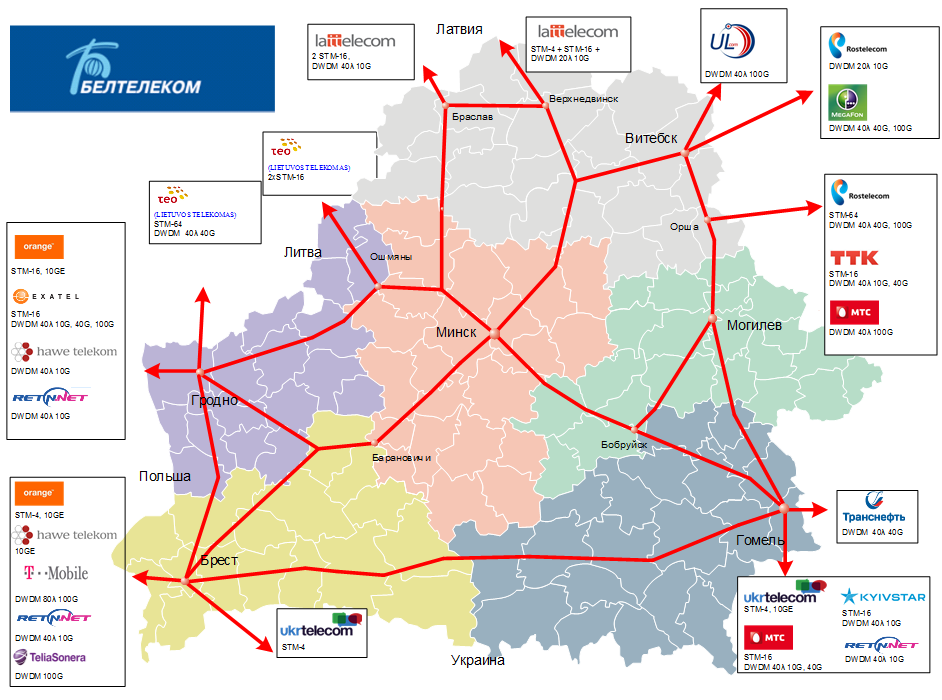
\includegraphics[width=\linewidth]{piersasnaja_setka.png}
    \caption{Першасная сетка на тэрыторыі Рэспублікі Беларусь}
\end{figure}

\vspace{-\baselineskip}
\subsection{Сеткі доступу}
Прадастаўленне паслуг стацыянарнай сувязі ў бліжэйшы перыяд будзе накіравана на захаванне існуючай абаненцкай базы і прадастаўленне дадатковых сэрвісаў. Сеткі РУП «Белтэлекам» будуць развівацца пераважна на базе платформы IMS. На пачатак 2019 года колькасць абанентаў платформы IMS склала больш за 2,9 млн. абанентаў.

IMS (англ. IP MultimediaSubsystem) - мультымедыйная падсістэма на базе IP - пратаколаў, якая з'яўляецца рашэннем для пераходу ад класічных тэлекамунікацыйных тэхналогій да IP - тэхналогій. IMS дазваляе распрацоўваць і прадастаўляць абанентам паслугі, заснаваныя на розных камбінацыях голасу, тэксту, графікі і відэа.

Новыя падыходы ў пытаннях пабудовы сетак доступу патрабуюць змяненняў у тым, што датычыцца канцавога абсталявання, якое ўстанаўліваецца на баку абанента. Для забеспячэння больш высокага пранікнення паслуг шырокапалоснага доступу, у тым ліку паслуг VoIP, у абанентаў усталёўваецца мадэм (хатні шлюз), абсталяваны разнастайнымі інтэрфейсамі (аналагавы тэлефонны порт, парты Ethernet. Порт Wi - Fi і інш) і забяспечвае прадастаўленне як галасавых паслуг (VoIP ), так і тэлематычных паслуг (доступ у Інтэрнэт, IPTV і інш).

У цяперашні час падключэнне абанентаў ажыццяўляецца з выкарыстаннем наступных тэхналогій:
\begin{enumerate}
    \item Вузлы аптычнай сеткі доступу на базе тэхналогіі GPON, якія будуюцца для прадастаўлення паслуг электрасувязі ўсім абанентам шматкватэрных дамоў, перш за ўсё ў гарадскіх населеных пунктах, а таксама ў кварталах дамоў новай індывідуальнай забудовы. На 1 студзеня 2019 года да сеткі GPON падключана больш за 2,2 млн. абанентаў РУП «Белтэлекам».
    \item Вузлы шырокапалоснага доступу тыпу DSLAM, якія ўводзяцца для прадастаўлення паслуг сувязі па праектах будаўніцтва сетак з выкарыстаннем медных кабеляў з мэтай эфектыўнага выкарыстання інвестыцый РУП «Белтэлекам», укладзеных у пабудаваную абаненцкую сетку, перш за ўсё на сельскіх сетках электрасувязі. Абаненцкая ёмістасць вузлоў DSLAM выкарыстоўваецца для прадастаўлення поўнага спектру шырокапалосных паслуг.
    \item Універсальныя вузлы доступу, якія забяспечваюць магчымасць ўстаноўкі ў іх абаненцкіх камплектаў з рознымі інтэрфейсамі: аналагавыя (POTS), шырокапалосныя медныя ADSL, VDSL-, SHDSL-інтэрфейсы, шырокапалосныя GPON інтэрфейсы. Дадзенае тэхнічнае рашэнне дазваляе на пераходны перыяд за кошт устаноўкі аднаго вузла доступу з адзінай кропкай падлучэння да сеткі перадачы дадзеных задавальняць попыт абанентаў на паслугі сувязі, на дадатковыя мультымедыйныя паслугі і прыкладанні, якія прадстаўляюцца платформай IMS, і інш.
\end{enumerate}

У 2011 годзе пачалося падключэнне па тэхналогіі GPON абанентаў РУП «Белтэлекам».  У пачатку 2019 года колькасць абанентаў, падключаных да сеткі GPON РУП «Белтэлекам» скалала  каля 2,2 млн. абанентаў, пры гэтым прырост за 2018 год склаў больш за 491,6 тыс. абанентаў.

Пры падключэнні абанентаў аптычны кабель пракладваецца непасрэдна да месцаў устаноўкі канцавога абаненцкага абсталявання. Такая тэхналогія прымяняецца не толькі пры будаўніцтве новых сетак доступу, але і пры мадэрнізацыі існуючых, напрыклад, пры вызваленні манціраванай ёмістасці АТС электроннага тыпу на гарадскіх сетках электрасувязі. Асноўнай мэтай абнаўлення ўжо існуючых сетак доступу з'яўляецца, перш за ўсё, неабходнасць паляпшэння якасці і пераліку прадастаўляемых паслуг за кошт пераключэння існуючых абанентаў шырокапалоснага доступу (xDSL) на новую тэхналогію (xPON).

Выкарыстанне тэхналогіі PON для будаўніцтва абаненцкага доступу дазваляе:
\begin{enumerate}
    \item забяспечыць абанентам шырокую паласу прапускання;
    \item пашырыць шырокавяшчальныя магчымасці;
    \item павялічыць даўжыню абаненцкай лініі аж да 20 км, аптымізаваць размеркавальную сетку і мінімізаваць яе энергаспажыванне (за кошт выкарыстання пасіўных аптычных разгалінавальнікаў);
    \item пашыраць дадатковыя сэрвісы і павялічваць хуткасці абмену трафікам перадачы дадзеных у залежнасці ад патрэбаў абанентаў;
    \item уніфікаваць працэс падключэння і абслугоўвання абанентаў за кошт мінімальнага выкарыстання актыўнага абсталявання.
\end{enumerate}

\subsection{Сеткі перадачы даных}
Першы крок у развіцці сеткі перадачы дадзеных Рэспублікі Беларусь быў зроблены ў 1992 годзе: у г.Мінску быў устаноўлены першы ў рэспубліцы электронны паштамт, і пачалося прадастаўленне паслугі электроннай пошты па пратаколе UUCP. Быў арганізаваны канал прапускной здольнасцю 19,2 Кбіт/с на маскоўскую кампанію «Релком».

Да 1995 года электронныя паштамты былі ўсталяваныя ва ўсіх абласных цэнтрах, паступова пашыраліся пулы дазвонкі для забеспячэння доступу абанентаў да паслугі.

У 1996 годзе было закуплена і ўстаноўлена ва ўсіх абласных цэнтрах і 12-ці найбуйнейшых раённых цэнтрах (усяго 18 вузлоў) абсталяванне, якое дазваляе прадастаўляць паслугі не толькі на базе камутаванага доступу, але і па выдзеленых лініях сувязі з хуткасцю да 64 Кбіт/с. Пачалася прапрацоўка пытання доступу Рэспублікі Беларусь да сеткі інтэрнэт.

У 1997 годзе на расійскую кампанію «Дэмас» быў арганізаваны канал прапускной здольнасцю 256 Кбіт/с. Пачалося прадастаўленне паслуг доступу да сеткі інтэрнэт.

1997 год - павялічваецца колькасць відаў доступу да сеткі перадачы дадзеных, пералік прадастаўляемых паслуг, прапускная здольнасць знешняга шлюза, удасканальваецца інфраструктура нацыянальнай сеткі перадачы дадзеных РУП «Белтэлекам». Запушчаны камутаваны парольны доступ, паслугі электроннай пошты POP3. Уведзены ў эксплуатацыю паслугі выдзеленага і паўпастаяннага доступу да сеткі інтэрнэт, закліканыя задаволіць патрэбнасць абанентаў у шырокапалосным доступ.

1999 год - арганізавана агульнарэспубліканская сістэма беспарольнага камутаванага доступу да сеткі інтэрнэт.

2002 - уведзены ў эксплуатацыю паслугі доступу ў сетку інтэрнэт па тэхналогіях ADSL і SHDSL.

Падзеяй 2006 года стала ўвядзенне новай гандлёвай маркі для паслуг шырокапалоснага доступу ў сетку Інтэрнэт - byfly (www.byfly.by).

У 2006-2007 гадах запушчана агульнарэспубліканская сетка MetroEthernet. Яе абсталяванне дазволіла дасягнуць прапускной здольнасці на сетцы перадачы дадзеных у аб'ёме 20Гбит/с на участках Мінск-Абласны цэнтр і 10 Гбіт/с на ўнутрыабласным узроўні.

2007 - масавы прырост абаненцкай базы byfly. У эксплуатацыю ўведзены першыя кропкі доступу па тэхналогіі Wi-Fi. Сетка Wi-Fi актыўна развіваецца ва ўсіх гарадах Беларусі.

2009 - увод у эксплуатацыю сеткі WiMax у г. Мінску.

У 2010 годзе пашырана прапускная здольнасць магістральнай сеткі перадачы дадзеных на участках Мінск - Абласны цэнтр да 40Гбит/с. Планамерна павялічвалася колькасць вузлоў сеткі перадачы дадзеных, у тым ліку ў невялікіх населеных пунктах і вёсках. На тарыфным плане byfly «Дамасед» 2 разы на працягу года двойчы расла хуткасць. Абнаўленне лінейкі тарыфных планаў byfly, паляпшэнне спалучэння цана/якасць. З'явіўся сацыяльны напрамак, byfly прапанаваў ільготныя тарыфныя планы для грамадзян з абмежаванымі магчымасцямі.

У 2011-2012 гадах праведзена поўная мадэрнізацыя цэнтральнага вузла перадачы дадзеных у г.Мінску з выкарыстаннем найноўшага высокатэхналагічнага абсталявання з падтрымкай інтэрфейсаў 100 Гбіт/с, якое дазволіла значна ўзмацніць і павялічыць існуючую ёмістасць ядра сеткі перадачы дадзеных.

У перыяд з 2012 года па 1-ы квартал 2013 года праведзены работы па мадэрнізацыі ўнутрыабласных сетак перадачы дадзеных з выкарыстаннем абсталявання DWDM, якое забяспечыла прапускную здольнасць перадачы трафіку на участках Абласны цэнтр-рэгіянальны цэнтр у аб'ёме ад 10 Гбіт/с, што павысіла якасць прадастаўлення існуючых паслуг перадачы дадзеных абанентам РУП "Белтэлекам".

У 2013-2014 гадах РУП «Белтэлекам» прадоўжаны работы па мадэрнізацыі ўнутрызонавых сетак перадачы дадзеных з выкарыстаннем абсталявання DWDM, у выніку чаго агульная прапускная здольнасць сетак склала больш за 1,1 Тбіт/с.

У 2013 годзе на сетцы перадачы дадзеных, у сувязі з вычарпаннем адраснай прасторы IPv4, укаранёна тэхналогія NAT44.

2014 год - пратакол IPv6 укаранёны на цэнтральным вузле і на магістральным узроўні Мінск-Абласныя цэнтры.

2016 год - выкананы работы па мадэрнізацыі абсталявання, якое забяспечвае прымяненне тэхналогіі NAT44.

У 2016-2017 гадах праведзены работы па мадэрнізацыі ўнутрыабласных сетак перадачы дадзеных, пашырана паласа прапускання каналаў у напрамку Мінск-Абласны цэнтр, Абласны цэнтр-рэгіянальны цэнтр.

2017 год - выкананы работы па мадэрнізацыі абсталявання тэрмінацыі (доступу да сеткі інтэрнэт) карыстальніцкіх сесій абанентаў гандлёвых марак Byfly і ЯСНА, што дазволіла забяспечыць прадастаўленне больш высакахуткасных тарыфных планаў канчатковым карыстальнікам.

\subsection{Тэлевізійнае і гукавое вяшчанне}
У рамках выканання «Дзяржаўнай праграмы ўкаранення лічбавага тэлевізійнага і радыёвяшчання ў Рэспубліцы Беларусь да 2015 года» прадугледжана будаўніцтва сеткі наземнага лічбавага эфірнага тэлебачання і арганізацыя лічбавага эфірнага тэлерадыёвяшчання на 93 радыётэлевізійных перадаючых станцыях. РУП «Белтэлекам» з 2005 года ажыццяўляў планавую мадэрнізацыю сеткі распаўсюджвання тэлевізійных праграм і будаўніцтва валаконна-аптычных ліній сувязі да дзеючых і зноў будуючыхся радыётэлевізійных перадаючых станцый. Пры гэтым прымянялася сучаснае абсталяванне, якое ажыццяўляе перадачу сігналу тэлеканалаў у лічбавым фармаце да лічбавых эфірных перадатчыкаў, устаноўленых на радыётэлевізійных перадаючых станцыях. У 2015 годзе РУП Белтэлекам» скончыў пракладку валаконна-аптычнага кабеля і падачу лічбавага агульнадаступнага пакета тэлевізійных праграм да ўсіх радыётэлевізійных перадаючых станцый рэспублікі, якія плануюцца да будаўніцтва. Сёння ажыццяўляецца дастаўка агульнадаступнага лічбавага пакета да 94 радыётэлевізійных перадаючых станцый, якія знаходзяцца на ўсёй тэрыторыі рэспублікі.

З 25 чэрвеня 2013 года РУП «Белтэлекам» пачаў рэалізацыю паслугі эфірнага камерцыйнага лічбавага тэлебачання. Прадастаўленне паслугі ажыццяўляецца пад гандлёвай маркай ZALA у выглядзе асобных пакетаў, якія ўключаюць 35 камерцыйных тэлевізійных каналаў стандарту DVB-T2 плюс агульнадаступны пакет. У цяперашні час ахоп насельніцтва Рэспублікі Беларусь эфірным камерцыйным лічбавым тэлебачаннем складае каля 95%.

Падрабязную інфармацыю паслугі па доступе да сеткі эфірнага лічбавага тэлевізійнага вяшчання і карты ахопу тэрыторыі глядзіце на сайце zala.by і beltelecom.by.

У сувязі з рэарганізацыяй РУП «Белтэлекам» і РУП «БРТПЦ шляхам далучэння да РУП «Белтэлекам» РУП «БРТПЦ», РУП «Белтэлекам» з трэцяга кастрычніка 2016 года вызначаны правапераемнікам правоў і абавязкаў РУП «БРТПЦ».

У цяперашні час РУП «Белтэлекам» забяспечвае перадачу па каналах сувязі тэлевізійных і радыёвяшчальных праграм тэлерадыёкампаній, арганізоўвае падачу пазапланавых тэлевізійных перадач, «відэамасты» і «відэаперагонаў» з месцаў правядзення мерапрыемстваў і іншых падзей, ажыццяўляе эфірную трансляцыю тэлевізійнага і гукавога вяшчання на тэрыторыі рэспублікі.

\subsection{Сеткі Wi-Fi}
РУП «Белтэлекам» з 2007 года развівае сетку шырокапалоснага бесправаднога доступу ў Інтэрнэт па тэхналогіі Wi-Fi.

У цяперашні час на сетцы РУП «Белтэлекам» устаноўлена і эксплуатуецца больш за 600 тыс. кропак доступу Wi-Fi. З іх больш за 3 тыс. кропак доступу Cisco Wi-Fi (SSID BELTELECOM) і каля 600 тыс. кропак доступу Home Wi-Fi (SSID byfly WIFI). Пункты доступу ўстаноўлены ў Нацыянальным аэрапорце Мінск, абласных аэрапортах рэспублікі, на аўтавакзалах, у гасцініцах, санаторыях, месцах грамадскага харчавання, гандлёвых цэнтрах, на рэспубліканскіх спартыўных аб'ектах, аўтазапраўках, у аддзяленнях банкаў і г.д.

У 2018 годзе запланавана далейшае пашырэнне сеткі больш чым на 2,5 тыс. кропак доступу Wi-Fi. У 2019 годзе таксама плануецца павялічыць колькасць пунктаў доступу больш чым на 2,5 тыс.

Доступ у сетку інтэрнэт для канчатковых карыстальнікаў у рамках гэтай сеткі рэалізаваны з дапамогай замовы на партале аўтарызацыі платных рэквізітаў доступу альбо па раней набытых пластыкавых картах. На сеткі Wi-Fi РУП «Белтэлекам» для карыстальнікаў дадаткова ўведзены азнаямленчы 30-хвілінны бясплатны доступ у інтэрнэт (1 раз у суткі для кожнага карыстальніка). Рэквізіты доступу карыстальнік атрымлівае з дапамогай SMS на пазначаны нумар тэлефона.

Акрамя нарошчвання тэхналагічнай магутнасці сеткі пільная ўвага надаецца развіццю і папулярызацыі бесправаднога доступу па тэхналогіі Wi-Fi.

На сённяшні дзень сеткі Wi-Fi шырока распаўсюджаныя. Абаненты прывыклі падлучацца да бясплатных сетак Wi-Fi у кафэ, гасцініцах і іншых месцах. Аднак часцяком уладальнікі кафэ, дробных гасцініц і іншых аб'ектаў, якія прадстаўляюць наведвальнікам бясплатны Wi-Fi, забываюць або не ведаюць пра Указ Прэзідэнта Рэспублікі Беларусь ад 01.02.2010 № 60, у адпаведнасці з якім правайдэр павінен ажыццяўляць захоўванне на працягу аднаго года інфармацыі пра карыстальнікаў сеткі інтэрнэт і падаваць яе ўпаўнаважаным органам.

РУП «Белтэлекам» прапануе юрыдычным асобам і індывідуальным прадпрымальнікам паслугі «Прадастаўленне ў карыстанне сеткі Wi-Fi» і «Прадастаўленне ў карыстанне аператарам існуючай інфраструктуры Wi-Fi», у рамках якіх забяспечвае выкананне ўсіх нарматыўных актаў.

Паслуга «Прадастаўленне ў карыстанне сеткі Wi-Fi» заключаецца ў арганізацыі і прадастаўленні ў карыстанне абаненту сеткі доступу ў інтэрнэт па тэхналогіі Wi-Fi. Сеткі Wi-Fi арганізуюцца на тэрыторыі гасцінічных комплексаў, гандлёва-выставачных цэнтраў і іншых аб'ектаў. Абаненту ствараецца сетка са сваім ідэнтыфікатарам SSID і наладжваецца партал аўтарызацыі ў адпаведнасці з яго фірмовым стылем. На сённяшні дзень ужо больш за 200 кампаній скарысталіся гэтай паслугай.

Паслуга «Прадастаўленне ў карыстанне аператарам існуючай інфраструктуры Wi-Fi» --- гэта паслуга сеткі перадачы дадзеных, якая прадугледжвае выкарыстанне інфраструктуры сеткі Wi-Fi РУП «Белтэлекам» іншымі аператарамі з мэтай прадастаўлення доступу ў сетку інтэрнэт сваім абанентам з аўтэнтыфікацыяй абанентаў па SIM-карце.

\subsection{Цэнтры апрацоўкі даных}
З 2006 года РУП «Белтэлекам» развівае ўласную сетку цэнтраў апрацоўкі дадзеных (ЦАД). Першы ЦАД, адкрыты ў чэрвені 2006 года ў Міжнародным цэнтры камутацыі (г. Мінск, вул. Захарава, 55), стаў першай хостынг-пляцоўкай у Беларусі.

Асноўныя характарыстыкі ЦАД:
\begin{enumerate}
    \item высокапрадукцыйнае камутацыйнае абсталяванне, якое забяспечвае перадачу дадзеных усярэдзіне цэнтра і абмен дадзенымі з вонкавымі сеткамі. Падключэнне сеткі ЦАД да сеткі Інтэрнэт ажыццяўляецца з двух ЦАД г. Мінска аптычнымі каналамі з сумарнай хуткасцю 160 Гбіт/с;
    \item высокапрадукцыйныя серверы;
    \item сетка захоўвання дадзеных на базе аптычных камутатараў і сістэмы захоўвання карпаратыўнага ўзроўню для захоўвання, рэзервавання і аднаўлення інфармацыі;
    \item прамысловая маштабуемая сістэма кандыцыяніравання;
    \item электрасілкаванне - 2 энергаўвода, 2 дызель-генератара, 6 крыніц бесперабойнага сілкавання;
    \item сістэма газавага пажаратушэння;
    \item кругласутачная сэрвісная падтрымка.
\end{enumerate}

Для забеспячэння далейшага развіцця ў 2007 годзе нашай кампаніяй рэалізаваны праект пабудовы цэнтраў апрацоўкі дадзеных ва ўсіх абласных гарадах Рэспублікі Беларусь. На базе абласных ЦАД аказваецца паслуга «Размяшчэнне абсталявання (colocation)», што дазваляе абанентам размяшчаць абсталяванне на спецыяльна абсталяваных хостынгавых пляцоўках у непасрэднай блізкасці ад свайго месцазнаходжання.

У снежні 2009 года была запушчана другая пляцоўка ЦАД у г. Мінску па вул. Убарэвіча, 8/2.

У 2014 годзе пашыраны цэнтральны ЦАД на вул. Захарава, 55: адкрыты тры серверных залы і адна інфраструктурная для размяшчэння крыніц бесперабойнага сілкавання. Дадатковыя плошчы для размяшчэння сервернага абсталявання аснашчаны найноўшымі сістэмамі электрасілкавання і сучаснай сістэмай чылернага кандыцыяніравання.

У ЦАД ажыццяўляецца кругласутачнае відэаназіранне. Доступ да ўласнага абсталявання арганізуецца толькі для ўпаўнаважаных спецыялістаў кампаній-партнёраў.

У цэнтры апрацоўкі дадзеных РУП «Белтэлекам» размяшчаюцца дзяржаўныя інфармацыйныя рэсурсы, рэсурсы і дадзеныя юрыдычных асоб і прыватных кліентаў. Магутнасці ЦАД таксама выкарыстоўваюць хостынг-аператары, у распараджэнні якіх - надзейныя сістэмы функцыяніравання абсталявання і кругласутачнае тэхнічнае суправаджэнне.
